The transport proxy's function is to negotiate and convert the media streams to allow for interoperation between WebRTC and enterprise communication endpoints. The specific problems related to this component are repeated below:

\begin{itemize}
\item{How to implement ICE?}
\item{How to negotiate the DTLS secret keys?}
\item{How to decrypt and encrypt the media streams from SRTP to RTP and reverse?}
\item{How to handle multiplexing and demultiplexing of the streams?}
\end{itemize}

%test web breaker for stun turn - look at ice candidates
%i'm not describing or testing crypto - why?
%dtls is basically tls for udp - won't go into that or the encryption/decryption part
%not looking for multiplexing in web breaker -why? Wireshark does not have great handling show screenshot/no rtcp) was not able to resolve packets as one rtcp stream

\section{ICE}
We could either implement our own solution or re-use the RTCWeb Breaker mentioned in section~\ref{sec:webrtc2sip} for this component. If we create our own transport proxy, we could either use Google's libjingle open-source C++ library\footnote{https://code.google.com/p/libjingle/} for doing P2P applications, or implement our own solution for doing ICE negotiations. The point is we need to speak the STUN and TURN protocols. By testing ICE in RTCWeb Breaker, I can evaluate if we can use the component for the proposed transport proxy.

Test setup is the same as in section \ref{sec:experiments} with Jitsi as the SIP client. In Wireshark I had to adjust a few settings to get all the RTP streams to show. In protocol preferences for RTP:
\begin{itemize}
\item Try to decode RTP outside of conversations: yes
\item Treat RTP version 0 packets: as STUN packets
\end{itemize}

\begin{figure}[here]
\centerline{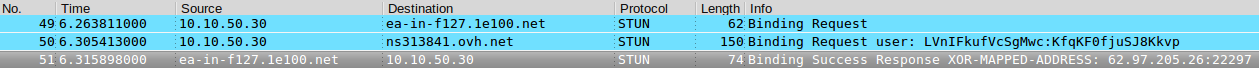
\includegraphics[width=\textwidth]{stun-success.png}}
\caption{Wireshark STUN activity}
\label{fig:wireshark-stun-activity}
\end{figure}

In Figure \ref{fig:wireshark-stun-activity} we can see that the WebRTC client sends a request to the STUN server (where do you see me?), and the STUN server answers with an IP address and port. This shows that ICE works properly in the RTCWeb Breaker.

\section{Encryption}
After we have handled ICE, we need to translate the media flows. VA communicates RTP and RTCP packets that needs to be encrypted. We do this by running a DTLS handshake that establishes a shared secret key between the peers, which is then reused as keying material within the encrypted media flows. I can evaluate that encryption works properly in RTCWeb Breaker, by looking for a DTLS handshake in Wireshark.

\begin{figure}[here]
\centerline{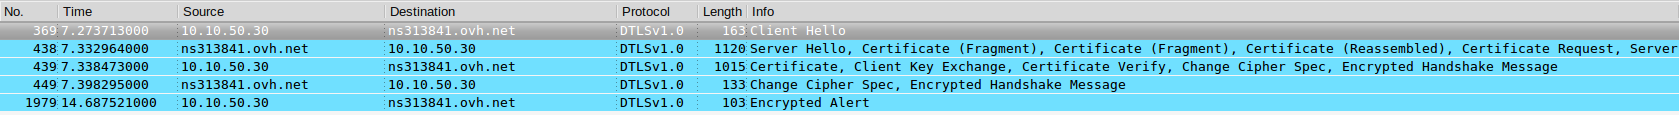
\includegraphics[width=\textwidth]{dtls-handshake.png}}
\caption{Wireshark DTLS activity}
\label{fig:wireshark-dtls-handshake}
\end{figure}

In Figure \ref{fig:wireshark-dtls-handshake} I have filtered out DTLS traffic. We can see a DTLS handshake with a secret key exchange. This shows that encryption works properly between the WebRTC client and the RTCWeb Breaker.

\section{Multiplexing}
Both RTP and RTCP require running on separate ports for each individual stream, which is a problem for clients running behind NATs and firewalls. Therefore we should support RTCP multiplexing and demultiplexing in this component. This enables delivery of both protocols over the same RTP session and port. In addition, WebRTC supports media multiplexing, so we should be able to support multiple streams running over the same single port. The webrtc2sip technical guide\footnote{http://webrtc2sip.org/technical-guide-1.0.pdf} says nothing about RTCWeb Breaker supporting multiplexing.

In Wireshark, sorting out the RTP streams revealed that there was multiplexing involved, but Wireshark did not handle multiplexing well, it could not resolve packets as one RTCP stream. There was a lot of ``Reserved for RTCP Conflict Avoidance'' packets running over the same ports as the media flows. This shows that the SRTP/SRTCP packets between the WebRTC client and RTCWeb Breaker were multiplexed. However, I could not find any evidence of media multiplexing. When I managed to transmit video in addition to audio, there were multiple connections spread over different ports like in Figure \ref{fig:wireshark-multiple-rtp-streams}. Keep in mind I'm running the experiment locally, so there are streams going in both directions here. The two distinctly (blue) marked streams are going from the WebRTC client to the RTCWeb Breaker.

\begin{figure}[here]
\centerline{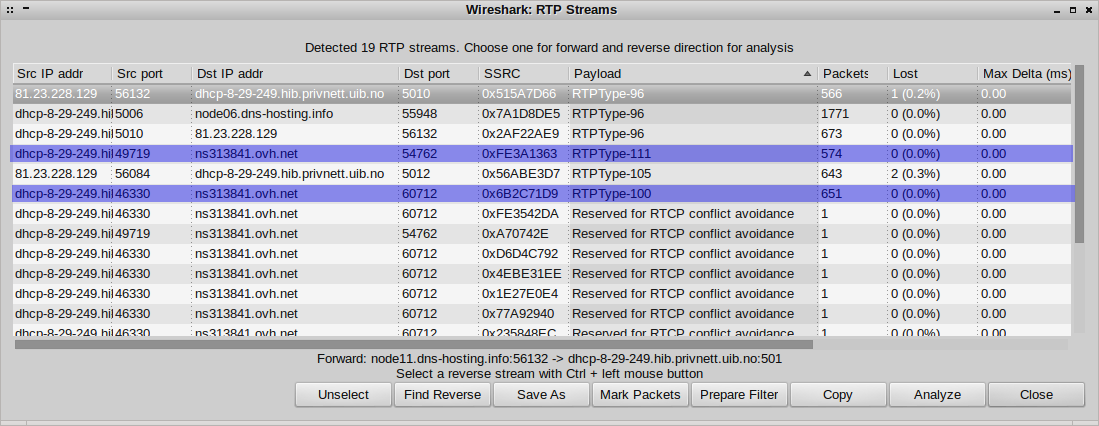
\includegraphics[width=\textwidth]{multiple-rtp-streams.png}}
\caption{Wireshark RTP streams}
\label{fig:wireshark-multiple-rtp-streams}
\end{figure}

\section{Summary}
By looking at the results of the experiments using RTCWeb Breaker, we can see that this module performs very well, the connections were smooth with low latency, and felt `live'. The RTCWeb Breaker seems to work exactly as it should. Both ICE end encryption worked properly with no problems. The calls went through instantly, with very little delay. This means that ICE found working candidates really fast. Multiplexing worked fine, but there was no evidence of media multiplexing. We can use the RTCWeb Breaker for our transport proxy, but we should add support for media multiplexing as well.